\documentclass{article}
\usepackage{tikz}
\usetikzlibrary{mindmap,trees}
\usepackage{verbatim}

\begin{document}

\pagestyle{empty}

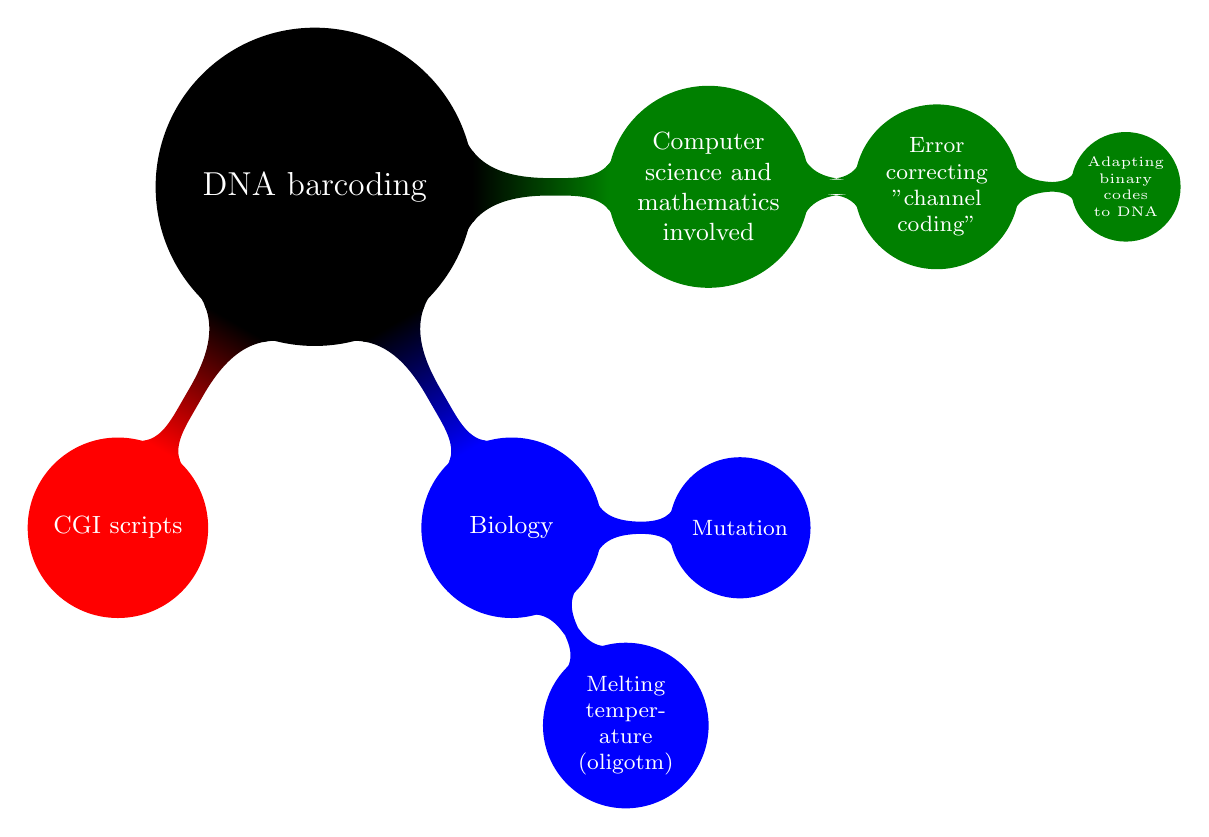
\begin{tikzpicture}
    \path[mindmap,concept color=black,text=white]
        node[concept] {DNA barcoding}
        [clockwise from=0]
        child[concept color=green!50!black] {
            node[concept] {Computer science and mathematics involved}
            child {
                node[concept] {Error correcting "channel coding"}
                child {
                    node[concept] {Adapting binary codes to DNA}
                }
            }
        }    
        child[concept color=blue] {
            node[concept] {Biology}
            child {
                node[concept] {Mutation}
            }
            child {
                node[concept] {Melting temperature (oligotm)}
            }
        }
        child[concept color=red] {
                node[concept] {CGI scripts}
        }
;\end{tikzpicture}

\end{document}
